\section{Background on Property Checking Methods}\label{sec:background}

In this section, we briefly sketch the verification methods for property checking that
we explore in our experiments. These are all well-established techniques and we refer 
the reader standard references for in-depth explanation~\cite{mc,hbmc}.
For clarity, we give bit-level descriptions of these verification techniques, but
many of them have analogues at word-level.

We group techniques into two classes, based on whether they use bit-level decision procedures 
or abstract domains. We call these \textit{SAT/SMT-based Verification} and 
\textit{Abstraction-based Verification}, respectively.

\subsection{SAT/SMT-based Verification}

The methods in this class are all used for experiments with both conventional verification tools,
operating on RTL designs, and verification of  our software netlist representation using software analysis tools.

\subsubsection{Bounded Model Checking} 

BMC~\cite{biere} is a bug-finding method that searches for bad states along a finite trace of 
the transition system. 
Given an unwinding `depth' $k$, BMC forms the logical characterization of a 
$k$-length chain of transitions along the transition relation $T$,  starting 
from any initial state satisfying $I[V_0]$. This is conjoined with a predicate saying that a bad state is encountered somewhere along the chain:

\begin{equation}\label{bmc-formula}
I[V_0] \wedge \bigwedge_{i{=}0}^{k{-}1}\delta[V_i, V_{i+1}] \wedge \bigvee_{i{=}0}^{k{-}1} \neg P[V_i]
\end{equation}

With BMC, this formula is checked for satisfiability using an efficient SAT procedure.
If found satisfiable, a chain of transitions into a bad state has been found;
a potential design bug---a violation of the safety property---has been uncovered.

\subsubsection{K-induction} 

BMC is incomplete: it searches for bad states only within a bounded trace of the system, 
which underapproximates the set of  all reachable states.  The method of 
$k$-induction addresses this problem~\cite{fmcad2000}.
  
In $k$-induction, we first use the BMC formula~(\ref{bmc-formula}) to check that the safety property
holds in all states reachable within $k$ steps from any initial state. This 'base case' of the induction will be established if SAT determines the formula is \textit{unsatisfiable}. We then check the step case below: 
%
\[\bigwedge_{i{=}0}^{k{-}1}\delta[V_i, V_{i+1}] \wedge \bigwedge_{i{=}0}^{k{-}1} P[V_i] \wedge \neg P[V_{k+1}] \]
%
If this formula is unsatisfiable, then no bad state is reachable from any sequence $k{+}1$ good states
allowed by the transistion system. This, together with the base case, confirm that no bad state is reachable from any initial state.

If the step case formula is satisfiable, then no conclusion about the property can be made. The method of k-induction then proceeds by restarting with a larger value of $k$. 
K-induction can be made complete by adding constraints that ensure any trace that satisfies the step case is 
loop-free~\cite{mc}.

%-------------------------------------------------------------------------------
\subsubsection{Interpolation-based Model Checking} 
%
Interpolation-based model checking~\cite{cav03} 
computes a step-wise overapproximation of the reachable state-space,
$Q$, for a fixed unrolling $k$ of $T$, which is shown as
follows.
%
\[ Q \wedge \delta_{k} \wedge P_{k+1} \implies P[V_{k+1}] \]
%
The value of $k$ is increased when the implication fails. This
progressively yields better overapproximation by 
generating an interpolant between the $i$-th 
overapproximation and $k$-step unrolling.
%which may be sufficient to prove the property $P$. 
Thus, the interpolation technique computes an abstraction 
of the postcondition with respect to the property $P$, 
by deriving interpolants from the failure of the
BMC problem.
%
Interpolation-based model checking is a complete method 
for reachability analysis of finite-state systems. 
%

%-------------------------------------------------------------------------------
\subsubsection{Predicate Abstraction with CEGAR}
%
This technique computes an abstract model $\hat{T}$ from the concrete model
$T$ using existential abstraction~\cite{cav97,cav2000}. 
%
Given a concrete state $x$ which is the 
valuation of all registers and a set of 
predicates, $Pred=\{\pi_{i} \ldots \pi_{k}\}$, 
an abstract state $b$ is obtained by applying 
an abstraction function $\alpha$, such that $b=\alpha(x)$.  
%
The abstract state $b$ is given by a vector 
of Boolean values of the predicates in $Pred$. 
%which is obtained by applying all the predicates 
%to the concrete state, 
%
Let $S$ be the set of concrete states in $T$. 
%
We define the abstract model given by, 
$\hat{T} = \langle \hat{I}, \pi, \hat{\delta} \rangle$.  
We define the components of $\hat{T}$ and property 
verification using predicate abstraction below. 
%
\begin{enumerate}
\item [A)] Transition Relation: $\hat{\delta} \mathrel{\hat{=}} \{(b,b') \mid \exists x,x' \in S: \delta(x,x') 
\wedge \alpha(x) = b \wedge \alpha(x') = b' \} $, $x=\{x_1 \ldots x_n\}, 
b=\{b_1 \ldots b_n\}, b_i=\pi_{i}(x) $, $\pi_i$ is the predicate on concrete variable $x_i$.

\item [B)] Initial State: $\hat{I}(b) \mathrel{\hat{=}} 
\exists x \in S: (\alpha(x) = b) \wedge I(x)$

\item [C)] Safety Property: $\hat{P}(b) \mathrel{\hat{=}} 
\forall x \in S: ((\alpha(x) = b) \implies P(x))$.  
Thus, if property $\hat{P}$ holds on all reachable states of the abstract model $\hat{T}$, then $P$ also holds on all reachable states of the concrete model $T$.
\end{enumerate}

%-------------------------------------------------------------------------------
\subsubsection{Property Directed Reachability} 
%
The property directed reachability~\cite{fmcad07} technique is briefly 
described as follows. 
% 
For any state $x$, let $\alpha_1(x), \alpha_2(x),\ldots,\alpha_n(x)$ be a 
sequence of inductive invariants generated by the PDR algorithm. Then, $P$ 
is an invariant of $T$ if the following conditions hold.
%
\begin{enumerate}
 \item [A)] $I(x) \implies P$
 \item [B)] $\forall i, I(x) \implies \alpha_i(x)$
 \item [C)] $\forall i, {\overset{k}{\underset{i=1}{\wedge}}} 
	 (\alpha_i(x) \wedge P(x) \wedge \delta(x,x') \implies \alpha_k(x'))$,
 $\alpha_k$ is inductive relative to $\alpha_1, \alpha_2,\ldots,\alpha_{k-1}$,
 \item [D)] $\forall i, {\overset{n}{\underset{i=1}{\wedge}}} 
	(\alpha_i(x) \wedge P(x) \wedge \delta(x,x') \implies P(x'))$, 
 $P$ is inductive relative to the inductive invariants $\alpha_1,\alpha_2,\ldots,\alpha_n$, 
\end{enumerate}
%  
The algorithm computes successive intermediate inductive invariants by 
removing the counterexamples-to-induction states in property-directed 
fashion.  Thus, the technique computes an overapproximation of the set of 
reachable states in successive steps until it finds an inductive 
strengthening assertion sufficient to prove the property. 


\begin{figure*}[tb]
\begin{center}
\small
\begin{tabular}{lcl} 
\hline\noalign{\vskip0.25ex}
\textbf{Verilog RTL} & \multicolumn{1}{l}{\textbf{Synthesized Hardware}} & \textbf{Software Netlist} \\
\hline
\begin{lstlisting}[boxpos=t,mathescape=true,language=Verilog,basicstyle=\scriptsize\ttfamily]
module top(clk, a, c, out); 
input clk , a;
output [1:0] c;
output reg [3:0] out;
reg b,e; reg [1:0] d;
initial begin
  b=0;d=2'b0;
  e=0;out=4'b0;
end
assign c = e ? 1'b0 : d; 
always @(posedge clk) 
begin
 b<=a;
 if(b) e <= b; 
 else  e <= 0; 
 d <= e + 1;
end
always @(posedge clk) 
begin
  out <= d*d;
end  
endmodule
\end{lstlisting}
&
\raisebox{-\totalheight}{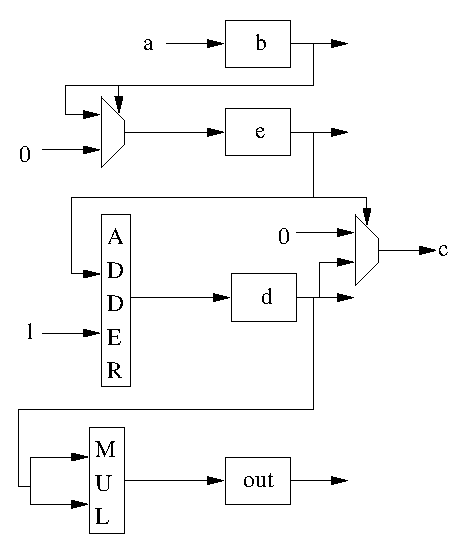
\includegraphics[width=0.28\textwidth]{figures/example/ckt_pspdftex.eps}}
&
\begin{lstlisting}[boxpos=t,mathescape=true,language=C,basicstyle=\scriptsize\ttfamily]
struct state_elements_top {
  unsigned int b,e;
  unsigned char d,out;
};
struct state_elements_top u1;

void top(unsigned int clk, 
 unsigned int a, 
 unsigned char *c, 
 unsigned char *out) {
 // shadow variables 
 unsigned int b_old = u1.b&0x1;
 unsigned char d_old = u1.d&0x3;
 unsigned int e_old = u1.e&0x1;
  
 u1.b = a;
 if(b_old) 
  u1.e = b_old&0x1;
 else
  u1.e = 0;
 u1.d = (e_old+1)&0x3;
 // update the output 
 u1.out = 
 (d_old&0x3) * (d_old&0x3);
 *out = u1.out&0xF;
 *c = u1.e ? 0 : (u1.d&0x3);
}
\end{lstlisting}\\
\hline
\end{tabular}
\caption{Translation of a Simple Circuit in Verilog HDL to a Software Netlist in C}\label{fig:example}
\end{center}
\end{figure*}



\subsection{Abstraction-based Verification}~\label{software-verif}
%
We now describe few well-known abstraction-based verification 
techniques that analyzes the transition system by computing an 
abstract pre-condition or abstract post-condition over a given 
abstract domain. Until now, the techniques described below 
are purely used in the context of software programs. In this paper, 
we employ these techniques for verifying the software netlist designs 
generated from the RTL. 
%-------------------------------------------------------------------------------
\subsubsection{Abstract Interpretation} 
%
Abstract Interpretation~\cite{Cousot92,CC79,DBLP:conf/emsoft/Cousot07},
is a theory of sound approximation of program semantics based on lattice 
structures. Static analysis using abstract interpretation is widely used 
to verify properties of safety-critical systems. 
%
In abstract interpretation, a given program is analyzed 
with respect to a given \textit{abstract domain} $\domain$.  
The technique computes an abstraction of the postcondition to derive an 
inductive invariant $AInv$.
%which includes the start state and is an 
%overapproximation of the set of reachable states.  
Elements of an abstract domain can be sets or conjuncts 
of formulae~\cite{DBLP:conf/vmcai/BrainDHGK13}.  
Given a transition system $T$, a set of formulas $A$ each of which is an 
element of $\domain$, and property $P$ as above, $AInv$ is computed as follows. 
%abstract interpretation can be described as follows. 
%
\begin{enumerate}
\item  $\exists AInv \in A. \forall x_0, x_1. (I(x_0) \implies AInv(x_0)) 
\wedge (AInv(x_0) \wedge \delta(x_0, x_1) \implies AInv(x_1))$, 
\item $\forall x. (AInv(x) \implies \neg{P(x)})$
\end{enumerate}
%
%where $A$ is the set of formulae each of which is the element of the 
%chosen abstract domain. The system is safe if there is no model. 
\Omit{
If an $AInv$ cannot the above conditions does not hold, the technique computes 
either a stronger invariant $AInv$ or choose a more expressive 
abstract domain to prove safety.
}
\Omit{
%-------------------------------------------------------------------------------
\subsubsection{Path-based symbolic execution}
%-------------------------------------------------------------------------------
%
Path-based symbolic execution is an well-known technique in program verification 
that is used for automatic test case generation~\cite{DBLP:conf/osdi/CadarDE08}.
Techniques based on precise forward symbolic 
execution~\cite{DBLP:conf/osdi/CadarDE08, King:1976:SEP:360248.360252}
executes a single path of a program at a time with symbolic inputs 
to generate symbolic expressions which are then conjoined with
the specification and are checked using a SAT/SMT solvers. 
The generated symbolic expression contains logical conjunction 
of the guards and assignments along that path.  This approach generates many 
SAT/SMT queries and may suffer from path explosion problem.

A similar technique is proposed for RTL in~\cite{star}. 
For sequential circuits, symbolic expressions contain path variables which 
are annotated by the time cycle to which it belongs. The 
work of~\cite{DBLP:journals/todaes/LiuV14} analyzes the 
feasibility of every path in the RTL program using a hybrid 
of concrete and symbolic execution and property based pruning.
}


%
%-------------------------------------------------------------------------------
\subsubsection{Automata based Trace Abstraction with Interpolants}
%-------------------------------------------------------------------------------
%
Automata-theoretic approaches to program verification~\cite{DBLP:conf/cav/KupfermanV00,
DBLP:books/sp/cstoday95/Vardi95,DBLP:conf/cav/HeizmannHP13} construct 
an automaton that represents a program together with its specification.
The negation of the specification is encoded via error locations in the automaton, 
that is, the error location is an accepting state.  The program satisfies the 
specification iff each trace accepted by the automaton is infeasible.
%
One of the automata-theoretic approaches for program verification 
is implemented in a tool called 
\textit{UltimateAutomizer}~\cite{DBLP:conf/tacas/HeizmannDGLMSP16}. 
The technique in~\cite{DBLP:conf/tacas/HeizmannDGLMSP16} decompose a 
program into sets of traces, and the decomposition is guided by proofs that 
are obtained for single traces. For correct programs, every non-empty set 
of error traces is an abstraction of the feasible error traces.  
%It obtains a proof for a single trace and trace abstraction generalizes 
%these proofs and combines them.  
Each iteration of the algorithm tries to obtain loop invariants for the path program
induced by the current counterexample.  This may be done through different techniques 
which can be applied iteratively. Each technique provides a set of Hoare triples that constitutes a proof of
safety for the current counterexample.
As soon as a technique yields loop invariants, the algorithm use these loop
invariants during the refinement and generalization step of trace abstraction.  If all the 
techniques have been exhausted and a loop invariant has not been obtained yet, the algorithm
use some or all (depending on the strategy) of the obtained hoare triples and 
refine or generalize with them.  Note that refinement reduces the number of error traces. 
